%----------------------------------------------------------------------------------------
%	PACKAGES AND OTHER DOCUMENT CONFIGURATIONS
%----------------------------------------------------------------------------------------

\documentclass[paper=a4, fontsize=11pt]{scrartcl} % A4 paper and 11pt font size

\usepackage[T1]{fontenc} % Use 8-bit encoding that has 256 glyphs
\usepackage{fourier} % Use the Adobe Utopia font for the document - comment this line to return to the LaTeX default
\usepackage[english]{babel} % English language/hyphenation
\usepackage{amsmath,amsfonts,amsthm} % Math packages

\makeatletter
%\renewcommand\thesection{}
%\renewcommand\thesubsection{\@arabic\c@section.\@arabic\c@subsection}
\makeatother

\usepackage{fancyhdr} % Custom headers and footers
\pagestyle{fancyplain} % Makes all pages in the document conform to the custom headers and footers
\fancyhead{} % No page header - if you want one, create it in the same way as the footers below
\fancyfoot[L]{} % Empty left footer
\fancyfoot[C]{} % Empty center footer
\fancyfoot[R]{\thepage} % Page numbering for right footer
\renewcommand{\headrulewidth}{0pt} % Remove header underlines
\renewcommand{\footrulewidth}{0pt} % Remove footer underlines
\setlength{\headheight}{13.6pt} % Customize the height of the header

%\numberwithin{equation}{section} % Number equations within sections (i.e. 1.1, 1.2, 2.1, 2.2 instead of 1, 2, 3, 4)
%\numberwithin{figure}{section} % Number figures within sections (i.e. 1.1, 1.2, 2.1, 2.2 instead of 1, 2, 3, 4)
%\numberwithin{table}{section} % Number tables within sections (i.e. 1.1, 1.2, 2.1, 2.2 instead of 1, 2, 3, 4)

%\setlength\parindent{0pt} % Removes all indentation from paragraphs - comment this line for an assignment with lots of text

\usepackage{graphicx}
\usepackage{caption}
\usepackage{subcaption}
\usepackage{algorithm2e}
\usepackage{booktabs}
\newcommand{\code}[1]{{\footnotesize\textsf{#1}}}
\newcommand{\q}[1]{``#1''}
\usepackage{listings}
\usepackage{geometry}
\geometry{letterpaper, margin=1.95cm}
\usepackage{url}
\usepackage{multirow}
%----------------------------------------------------------------------------------------
%	TITLE SECTION
%----------------------------------------------------------------------------------------
\newcommand{\horrule}[1]{\rule{\linewidth}{#1}} % Create horizontal rule command with 1 argument of height
\title{	
\normalfont \normalsize 
\textsc{Utah State University, Computer Science Department} \\ [25pt] % Your university, school and/or department name(s)
\horrule{0.5pt} \\[0.4cm] % Thin top horizontal rule
\huge CS5890 Data Science - Project Checkpoint \\ Random Acts Of Pizza \\ % The assignment title
\horrule{2pt} \\[0.5cm] % Thick bottom horizontal rule
}
\author{Team \textbf{Pizza Hackers}: Tam Nguyen and Hung Pham} % Your name
\date{\normalsize\today} % Today's date or a custom date
\begin{document}
\maketitle

\section{Introduction}

In this checkpoint we will discuss our current finding on a social interaction dataset, where requester ask for free pizza on a Reddit community \q{Random Acts of Pizza}\footnote{\url{https://www.reddit.com/r/Random_Acts_Of_Pizza/}}. We will show that predicting the outcome of request using just the requester information is not possible and the actual textual content of the request provide much more useful information that can be used to perform good prediction. We also performed a basic empirical analysis of words using contrast mining and found that certain words indicate \q{positive} effect on the outcome while other demonstrate a \q{negative} effect. Finally, we will discuss our next steps including using more sophisticate un-supervised learning (topic modeling and word2vec\footnote{Tomas Mikolov, Ilya Sutskever, Kai Chen, Greg S Corrado, Jeff Dean. \emph{Distributed representations of words and phrases and their compositionality}, Advances in neural information processing systems, 2013.}) to create our features, as well as more effective classifier model (Support Vector Machine).

\section{The dataset}
As mentioned in the proposal. The dataset consists of 4040 requests collected from the Reddit community Random Acts of Pizza between December 8, 2010 and September 29, 2013. Each data object is a request for a free pizza. There are 994 requests received a pizza while 3046 requests did not. We converted the dataset from JSON into data frames in \texttt{R}, each row in a data frame represents a request while each column represents an attribute. Attributes include information about requests such as id, text, requester name, etc. and meta-data such as: time of the request, activity of the requester, community-age of the requester, etc. We removed fields that contain values collected after the time a request was posted. Table \ref{fields} shows important attributes (and explanations that) we consider in our analysis.

\begin{table}[]
	\sf\scriptsize
	\centering
	\caption{Important attributes used in our analysis}
	\label{fields}
	\begin{tabular}{lp{10cm}}
		\toprule
		Important Attributes                              & Explanations                                                                          \\
		\midrule
		\multicolumn{2}{l}{Request text}                                                                                                        \\
		\midrule
		request\_title                                    & Title of the request                                                                  \\
		request\_text\_edit\_aware                        & Request text after removing comments indicating the success of the request            \\
		\midrule
		\multicolumn{2}{l}{Requester information}                                                                                                 \\
		\midrule
		requester\_account\_age\_in\_days\_at\_request    & The age of requester (in days) at time of request                                     \\
		requester\_number\_of\_comments\_at\_request      & The number of comments on Reddit by requester at time of request                      \\
		requester\_number\_of\_posts\_at\_request         & The number of posts on Reddit by requester at time of request.                        \\
		requester\_subreddits\_at\_request                & The number of subreddits that requester had posted in at the time of request. \\
		requester\_upvotes\_minus\_downvotes\_at\_request & Difference of upvotes and downvotes of requester at time of retrieval.                \\
		requester\_upvotes\_plus\_downvotes\_at\_request  & Sum of  upvotes and downvotes of requester at time of request.                        \\
		\bottomrule
	\end{tabular}
\end{table}
\section{Analysis on requester information}
In this section, we perform analysis on requester information attributes. Such analysis will give us some idea of how the information available in Reddit about the requesters could effect whether a request receive a pizza.

\subsection{Contrast analysis}
In our first analysis, we perform comparison between successful and unsuccessful requests on each requester information attribute. For example, with the attribute \textit{requester\_account\_age\_in\_days\_at\_request}, we want to see whether an older account holder will have more chance at receiving a free pizza or not. In order to do that, for each attribute, we collect values associate with successful and unsuccessful requests and visualize them for comparison. To have more precise analysis and better visualization, we removed outliers by dropping all value that are ``too extreme''. We used the standard rule to identify outliers. A value is considered as outliers if it greater than $1.5 \times IQR$ above the third quantile or less than $1.5 \times IQR$ below the first quantile. Figure \ref{boxplot} shows boxplots of requester information attributes based on the success of requests. We can see that, the median values for successful requests are slightly higher than for unsuccessful requests for all analyzed attributes but the there is not much different between the range of values and the shape of box plots. This result suggests that the requester information attributes do not have much predictive power because the distributions of attribute values are similar in both successful and unsuccessful requests.
 
\begin{figure}
	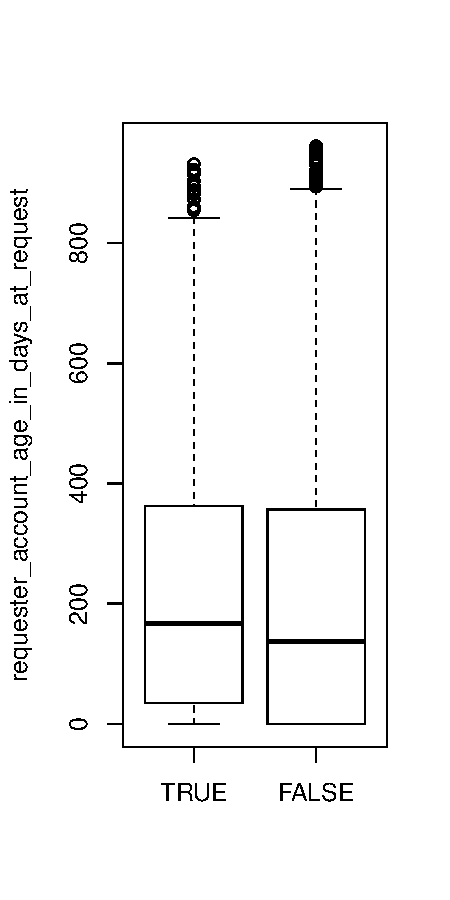
\includegraphics[width=0.16\textwidth]{data/requester_account_age_in_days_at_request}
	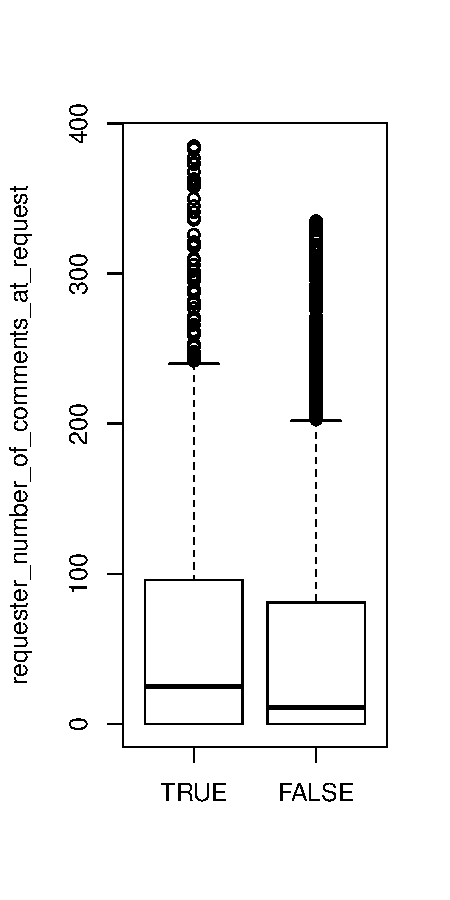
\includegraphics[width=0.16\textwidth]{data/requester_number_of_comments_at_request}
	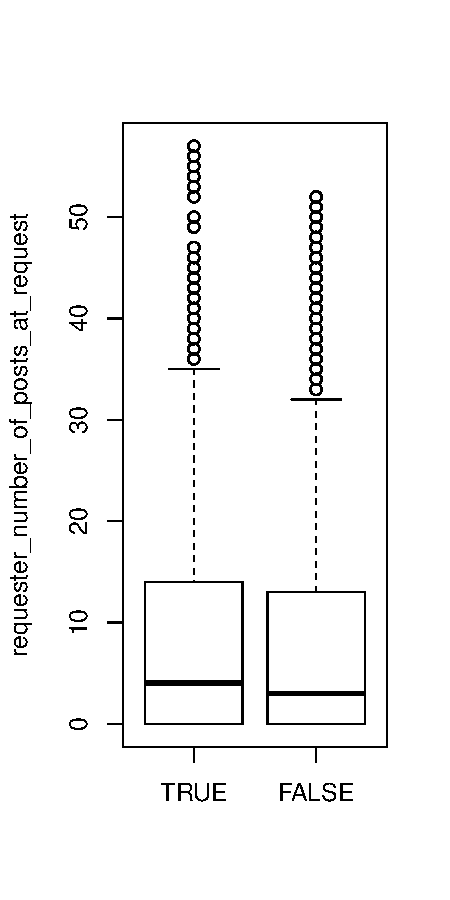
\includegraphics[width=0.16\textwidth]{data/requester_number_of_posts_at_request}
	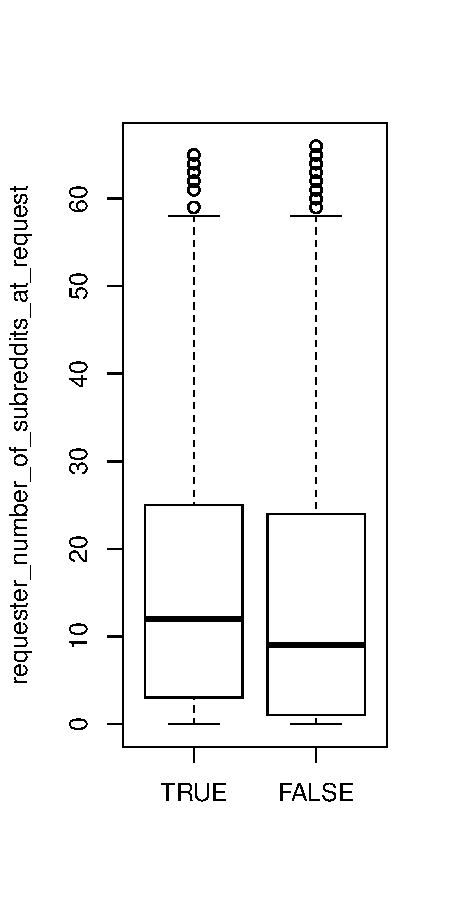
\includegraphics[width=0.16\textwidth]{data/requester_number_of_subreddits_at_request}
	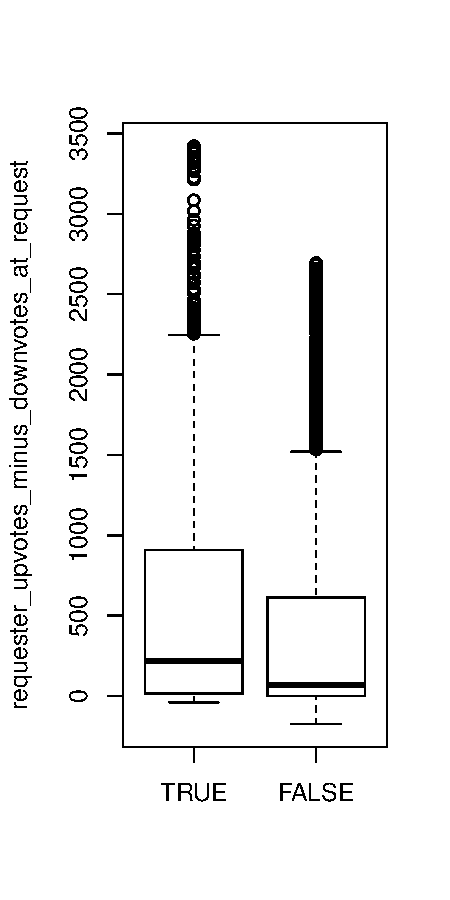
\includegraphics[width=0.16\textwidth]{data/requester_upvotes_minus_downvotes_at_request}
	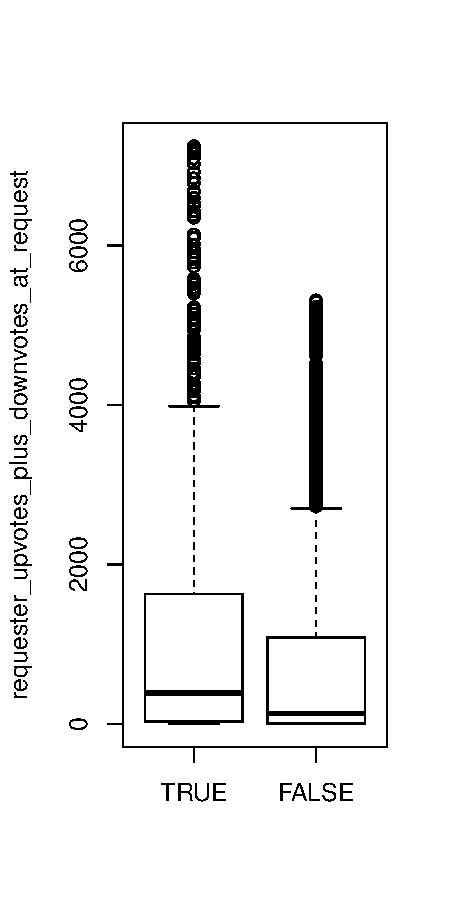
\includegraphics[width=0.16\textwidth]{data/requester_upvotes_plus_downvotes_at_request}
	\vspace*{-0.6cm}
	\caption{Boxplots of requester information attributes based on the success of requests}
	\vspace*{-0.6cm}
	\label{boxplot}
\end{figure}

\begin{table}[]
	\centering
	\caption{The confusion matrix for a fold in the cross validation}
	\label{confusion1}
	\begin{tabular}{|c|c|c|c|}
		\hline
		\multicolumn{2}{|c|}{\multirow{2}{*}{}}                & \multicolumn{2}{c|}{Actual}                            \\ \cline{3-4} 
		\multicolumn{2}{|c|}{}                                 & \multicolumn{1}{c|}{TRUE} & \multicolumn{1}{c|}{FALSE} \\ \hline
		\multicolumn{1}{|c|}{\multirow{2}{*}{Predict}} & TRUE  & 0                         & 0                          \\ \cline{2-4} 
		\multicolumn{1}{|c|}{}                         & FALSE & 92                        & 312                        \\ \hline
	\end{tabular}
	\vspace*{-0.6cm}
\end{table}

\subsection{Outcome prediction}
In second analysis, we perform a request classification task using requester information attributes to verify our assumption. There are several prediction models can be used in this classification task such as decision trees, logistic regression, SVM, etc. In our experiment, we used a simple logistic regression as the prediction method. We also used $10$-fold cross validation to measure the accuracy of the prediction model. At the iteration $i$ in the cross validation, we used fold $i$ as test set and the remaining data as training set. To measure the accuracy of the prediction model, we used the $F$-measure\footnote{\url{https://en.wikipedia.org/wiki/F1_score}}. The overall $F$-measure is 0. The reason why the value of the $F$-measure is zero is that the classifier always predict that a request will not receive a pizza. Table \ref{confusion1} show here a confusion matrix in a fold of the cross validation. We can see that the classifier predict \texttt{FALSE} values. From the experiment, we see that prediction models based requester information attributes do not perform well. It suggests that the decision whether or not a request receive a pizza do not based on the information about requester.


\section{Analysis on request textual content}
In this section, we perform analysis on the two text-based attributes in our dataset, i.e. \textit{request\_title} and \textit{request\_text\_edit\_aware}. These attributes contain the title and textual body of each request. Most of decision will be based upon the contents of these two attributes.

\subsection{Textual content preprocessing}

In order to perform analysis, we need to do preprocessing steps on these two attributes. First, we observed that the title of a request somewhat summaries the content in the request text, thus, analyze these two text attributes separately it is a good idea to combine title and the request text in to a single text document. Next, we tokenized a document into words using simple regular expression to find words: \verb|[a-z][a-z'\-_]+[a-z])||\verb|([a-z]+)|. In language, there are several stop words which are words that have meaning too general e.g.\texttt{you, me}, etc. These words ofter do not have predictive power because they occur in both successful and unsuccessful requests. Thus, after tokenizing words, we removed stop words from documents. After stop words removal step, there are 12930 distinct words occur in the corpus, 6358 distinct words only occur in successful requests, and 10823 distinct words only occur in unsuccessful requests.     

\subsection{Empirical analysis on words}

When looking at request text, we are often interested in keywords or topics that are associated with successful requests and unsuccessful requests. These keywords can give some insights about which kind of requests often receive pizza and which kind of requests do not. We defined ``positive'' keywords as the words that often occur in successful request but rarely occur in the unsuccessful requests, and ``negative'' keywords as the words that often occur in unsuccessful request but rarely occur in the successful requests. To find top ``positive'' words, we ranked all words based on \textit{constract score}:

\begin{equation}
	\phi = \frac{p}{n}(p-n)
\end{equation}    

where $p$ and $n$ are correspondingly the counts of successful and unsuccessful requests containing the word. After compute \textit{constract score}, we can select top-$k$ words based on the ranking of scores. The process of finding top ``negative'' words as similar but in the \textit{constract score} formula we exchange $n$ and $p$. Figure \ref{top} shows top-30 ``positive'' words and ``negative'' words. From the figures, there are several interesting points we can see. Top ``positive'' words contains several words related to children topic like \texttt{\{disney, daughter's, babies\}}, location topic like \texttt{\{toledo, wellington, asian\}}. This suggests that requests mentioned about those topics tend to be successful. Top ``negative'' words contains several words related to money topic like \texttt{\{money, penny, penniless\}}, relationship topic like \texttt{\{love, friend, girlfriends, coworkers\}}, bad activities like \texttt{\{frunk, smoking, broke, dumped\}}, and locations like \texttt{\{island, alaska\}}. This suggests that requests mentioned about those topics tend to be unsuccessful.

\begin{figure}
	\centering
	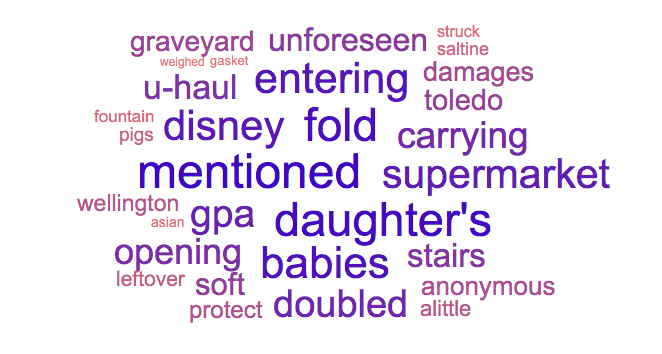
\includegraphics[width=0.40\textwidth]{data/positive}
	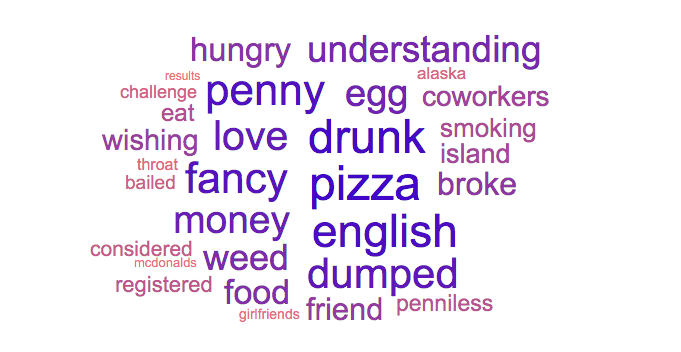
\includegraphics[width=0.40\textwidth]{data/negative}
	\caption{Top ``positive'' words and top ``negative'' words}
	\label{top}
\end{figure}

\subsection{Outcome prediction}
In second analysis, we perform a classification task using text attributes. For the prediction model, we built the same logistic regression model (maximum entropy classifier) as the model for requester information attributes. We also used the same cross validation settings and folds as the previous classification experiment. Table \ref{confusion2} shows a confusion matrix for the same fold as the previous experiment but now using text attributes. In the result, the overall $F$-measure are \textbf{0.31}. The result now is much better than using requester information attributes. The classifier now can classify both successful and unsuccessful request.

 \begin{table}[]
	\centering
	\caption{The confusion matrix for a fold in the cross validation (using text attributes)}
	\label{confusion2}
	\begin{tabular}{|c|c|c|c|}
		\hline
		\multicolumn{2}{|c|}{\multirow{2}{*}{}}                & \multicolumn{2}{c|}{Actual}                            \\ \cline{3-4} 
		\multicolumn{2}{|c|}{}                                 & \multicolumn{1}{c|}{TRUE} & \multicolumn{1}{c|}{FALSE} \\ \hline
		\multicolumn{1}{|c|}{\multirow{2}{*}{Predict}} & TRUE  & 27                         & 79                          \\ \cline{2-4} 
		\multicolumn{1}{|c|}{}                         & FALSE & 33                        & 265                        \\ \hline
	\end{tabular}
\end{table} 

%\section{Vector representation of words}
\section{Next steps}

In this section we will discuss our next steps, what we think we will try based on the current finding. According to the current result, textual content of each request provide a good source of information that we want to explore further. We have tried to used a simple bag of word model as input for our logistic regression, however, this is not the best possible approach.\\

Recently more effective un-supervised techniques such as topic modeling or vector space representation (word2vec) have emerged. Not only such techniques could improve our prediction accuracy, they would also help us under stand more in details the kind of request that have the most successful rate. For example, topic modeling would help us cluster word or phrases into different topics and by analyze the weight assigned by logistic regression to each topic, we will see which of the topics are more important in creating a successful request.\\

Vector space representation has been applied very successful in the field of natural language processing. In particular, word2vec has gained popularity due to it simplify and the fact that the tool was made available by Google. The idea is that word2vec will encored each word as a \q{semantic} vector, with the similar vectors represent similar word (e.g. apple and orange will be similar because they are both fruits), not only that these vector also display very interesting linear sub-structure (e.g. vector(queen)-vector(woman)+vector(man) is similar to vector(king)). We hope that with this \q{semantic} encoding our prediction will be much stronger.\\

Last but not least, we plan to use a more sophisticate classifier, namely Support Vector Machine (SVM). This classifier will provide much more generalized model that will help increase the overall accuracy.

%\begin{thebibliography}{10}
%
%\bibitem{tim14}
%Tim Althoff, Cristian Danescu-Niculescu-Mizil, Dan Jurafsky.
%\emph{How to Ask for a Favor: A Case Study on the Success of Altruistic Requests},
%Proceedings of ICWSM,
%2014.
%
%\bibitem{word2vec}
%Tomas Mikolov, Ilya Sutskever, Kai Chen, Greg S Corrado, Jeff Dean.
%\emph{Distributed representations of words and phrases and their compositionality},
%Advances in neural information processing systems,
%2013.


%\end{thebibliography}

\end{document}